% Usa pacote da FURG MPU
\documentclass{furgmpu}
% Língua do texto
\usepackage[brazilian]{babel}
% Muda título das referências
\addto{\captionsbrazilian}{\renewcommand{\refname}{REFERÊNCIAS}}
% Definindo comando \palavraschave
\newcommand{\palavraschave}[1]{\noindent\textbf{Palavras-chave:} #1.\vspace{0.2cm}\renewcommand{\baselinestretch}{1.07}}

% Título do trabalho
\titulo{TÍTULO DO TRABALHO: SUBTÍTULO}

% Autores
\autores{
	% Aqui vão os autores/alunos
	% Colocar 2 por linha, separados por ponto e vírgula
	SOBRENOME, Prenome; SOBRENOME, Prenome;\\
	SOBRENOME, Prenome (autor 3).
}{
	% Aqui vão os orientadores
	SOBRENOME, Nome
}{
	% E-mail do primeiro autor
	email@email.com
}{
	% Instituição dos autores
	Instituição
}

% Começo do documento
% O trabalho deverá ter entre 2 e 4 páginas
\begin{document}
\maketitle

% Use de 3 a 5 palavras chave separadas por ponto e vírgula
\palavraschave{Palavra-chave 1; Palavra-chave 2; Palavra-chave 3; Palavra-chave 4; Palavra-chave 5}

\section{INTRODUÇÃO}

Aqui deve ser apresentada uma breve contribuição teórica. A introdução de um trabalho se destina a apresentar o tema abordado. Esta seção deve conter os objetivos propostos, o problema/hipótese (quando for o caso) e a justificativa.

\section{METODOLOGIA}

Apresentar, de forma sucinta, os materiais e métodos utilizados, tais como: método empregado, universo, população e amostra, técnicas, instrumentos e procedimentos de coleta de dados e procedimentos de análise. Citando \cite{exemplo01} e \cite{exemplo02}.

\section{RESULTADOS E DISCUSSÃO}

Os resultados devem ser apresentados de forma clara. Se forem dados parciais, devem constar no texto.

Qualquer que seja o tipo de ilustração, sua identificação aparece na parte superior, precedida da palavra designativa (desenho, esquema, fluxograma, fotografia, gráfico, mapa, organograma, planta, quadro, retrato, figura, imagem, entre outros), conforme exemplo da Figura \ref{fig:exemplo}. Após a ilustração, na parte inferior, indicar a fonte consultada.

\begin{figure}[ht]
	\centering
	\caption{Site da FURG.}
	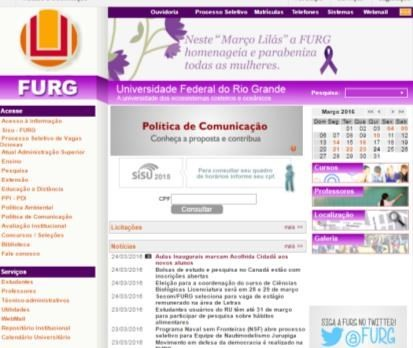
\includegraphics[width=4.13cm,scale=1]{img.jpg}\\
	\mbox{Fonte: O(s) autor(es).}
	\label{fig:exemplo}
\end{figure}

As tabelas apresentam informações tratadas estatisticamente, para tal, deverá ser seguida recomendação da ABNT NBR 14724 Trabalhos acadêmicos – apresentação (2011), para uso das normas de apresentação tabular, do IBGE (1993).

\begin{table}[ht]
	\centering
	\caption{Dados de ingresso}
	\begin{tabular}{cc}
		\toprule
		\textbf{\textit{Curso}} & \textbf{\textit{Dados}} \\
		\midrule
		Curso 1 & Dados de ingresso 1\\
		Curso 2 & Dados de ingresso 2\\
		\bottomrule
	\end{tabular}
	\label{tab:tabela}
\end{table}

\section{CONSIDERAÇÕES FINAIS}

Apresentar de forma sucinta as reflexões realizadas até o momento, os aspectos relevantes sobre o trabalho e as recomendações que se façam necessárias.

% Referências
\titlespacing{\section}{0pt}{24pt}{12pt}\bibliography{ref}

\end{document}
